\documentclass{beamer}
\usepackage{relsize}
\usepackage{color}

\usepackage{listings}
\usetheme{CambridgeUS}
%\usepackage{beamerthemesplit} % new 
\usepackage{enumitem}
\usepackage{amsmath}                    % See geometry.pdf to learn the layout options. 
\usepackage{amsthm}                   % See geometry.pdf to learn the layout options. There 
\usepackage{amssymb}                    % See geometry.pdf to learn the layout options. 
\usepackage[utf8]{inputenc} 
\usepackage{graphicx}
\usepackage[english,bulgarian]{babel}

\lstset{language=C++,
                basicstyle=\ttfamily,
                keywordstyle=\color{blue}\ttfamily,
                stringstyle=\color{red}\ttfamily,
                commentstyle=\color{green}\ttfamily,
                morecomment=[l][\color{magenta}]{\#}
}

\newtheorem{mydef}{Дефиниция}[section]
\newtheorem{lem}{Лема}[section]
\newtheorem{thm}{Твърдение}[section]

\DeclareMathOperator{\restrict}{\upharpoonright}

\setitemize{label=\usebeamerfont*{itemize item}%
  \usebeamercolor[fg]{itemize item}
  \usebeamertemplate{itemize item}}

\setbeamercovered{transparent}



\begin{document}
\title[Структури от данни и програмиране]{Речници: Хеш таблици и Trie} 
\author{Калин Георгиев} 
\frame{\titlepage} 

\section{Речници} 


\begin{frame}
\centerline{Речници}
\end{frame}


\begin{frame}[fragile]
\frametitle{Речник}
\begin{center}
\begin{tabular} {c | l}
  cat & a small animal that is related \\
      & to lions and tigers and that is \\
      & often kept by people as a pet \\
      \hline\\
  dog & canid; especially :  a highly variable \\
      & domestic mammal (Canis familiaris) closely \\
      & related to the gray wolf
\end{tabular}  
\end{center}
\end{frame}

\begin{frame}[fragile]
\frametitle{``Номератор'' на ключови думи}
\begin{center}
\begin{tabular} {c | l}
  if & 0 \\
      \hline\\
  then & 1 \\
      \hline\\
  else & 2 \\
      \hline\\
  for & 3 \\
      \hline\\
  ... & ... \\
      \hline\\
\end{tabular}  
\end{center}
\end{frame}

\begin{frame}[fragile]
\frametitle{Променливи на средата}

\begin{columns}[t]
  \begin{column}{0.5\textwidth}
\begin{flushleft}
\relscale {0.7}
\begin{lstlisting}
 var x = 10;
 var y = "Hello"; 
\end{lstlisting}
\end{flushleft}
  \end{column}

  \begin{column}{0.5\textwidth}
\begin{flushleft}
\begin{tabular} {c | l}
  x   & 10 \\
      \hline\\
  y & ``hello''

\end{tabular}  
\end{flushleft}

  \end{column}
\end{columns}


\begin{columns}[t]
  \begin{column}{0.5\textwidth}
\begin{flushleft}
\relscale {0.7}
\begin{lstlisting}
 var x = 10;
 var y = "Good bye!"; 
\end{lstlisting}
\end{flushleft}
  \end{column}

  \begin{column}{0.5\textwidth}
\begin{flushleft}
\begin{tabular} {c | l}
  x   & 10 \\
      \hline\\
  y & ``Good bye!''

\end{tabular}  
\end{flushleft}

  \end{column}
\end{columns}


\end{frame}


\section{Хеш таблици} 

\begin{frame}
\centerline{Хеш таблици}
\end{frame}



\begin{frame}[fragile]
\frametitle{Илюстрация на хеш таблица}
\begin{center}
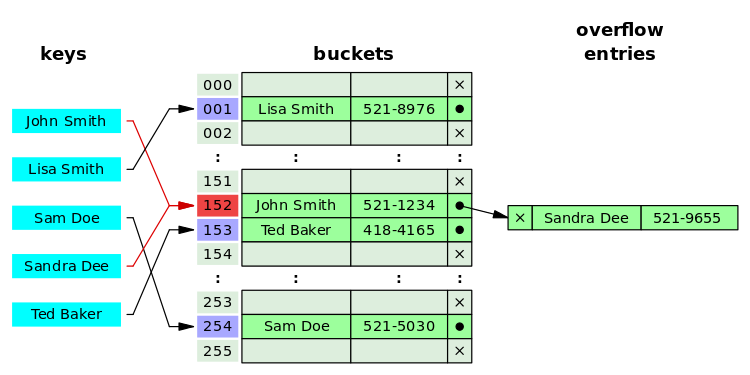
\includegraphics[width=11cm]{images/hast1}
  
\end{center}
\begin{center}
\relscale{0.5}
Източник: Wikipedia
\end{center}
\end{frame}




\begin{frame}[fragile]
\frametitle{Основни елементи}


\begin{columns}[t]
  \begin{column}{0.4\textwidth}

\relscale{0.9}
\begin{itemize}
  \item Хеш функция

  $h:Keys \rightarrow [0;n)$

  $h(\text{``John Smith''})=152$

  \item Колизии
  
  $k_1 \neq k_2$, $h(k_1)=h(k_2)$

  \item {Примерна хеш фунцкия за низ}

  $h(s)=|\sum\limits^{i=0}_{strlen(s)-1}(int)s_i|_n$
\end{itemize}

  \end{column}
  \begin{column}{0.6\textwidth}

\begin{center}
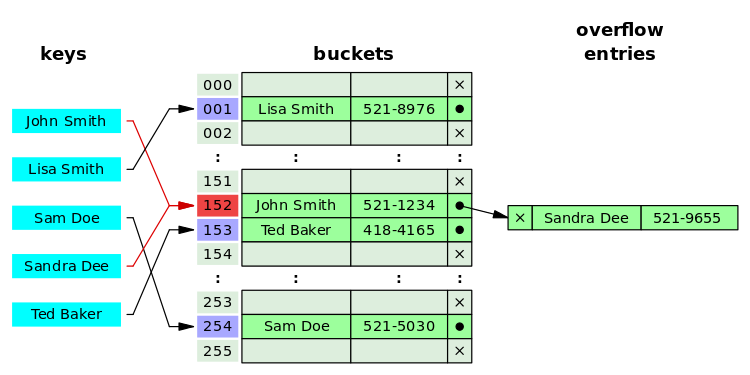
\includegraphics[width=7cm]{images/hast1}  
\end{center}
\begin{center}
\relscale{0.3}
Източник: Wikipedia
\end{center}

  \end{column}
\end{columns}
\end{frame}

\section{Trie}


\begin{frame}
\centerline{Trie}
\end{frame}


\begin{columns}[t]
  \begin{column}{0.20\textwidth}


  	\begin{tabular}{c | c}
  		\textit{key} & \textit {value} \\\hline
  		to & 7 \\
  		tea & 3 \\
  		ted & 4 \\
  		ten & 12 \\
  		A & 15 \\
  		i & 11 \\
  		in & 5 \\
  		inn & 9 \\
  	\end{tabular}

  \end{column}
  \begin{column}{0.80\textwidth}
	\begin{center}
	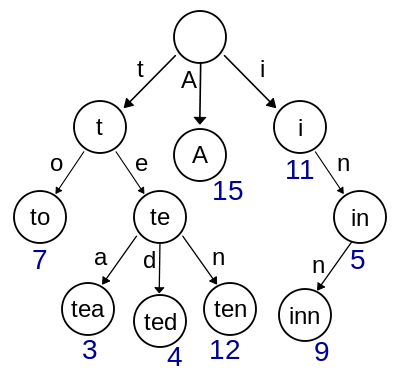
\includegraphics[width=5cm]{images/trie}  
	\end{center}
	\begin{center}
	\relscale{0.3}
	Източник: Wikipedia
	\end{center}

  \end{column}
\end{columns}

\begin{itemize}	
	\item Няма колизии
	\item Няма нужда от рехеширане
	\item Ползволява итериране по наредба на ключовете
\end{itemize}	



\begin{frame}
\centerline{Въпроси?}
\end{frame}


\end{document}

\begin{columns}[t]
  \begin{column}{0.55\textwidth}

  \end{column}
  \begin{column}{0.45\textwidth}

  \end{column}
\end{columns}


